\documentclass{standalone}

\usepackage{tikz}
\usetikzlibrary{calc, intersections}


\begin{document}
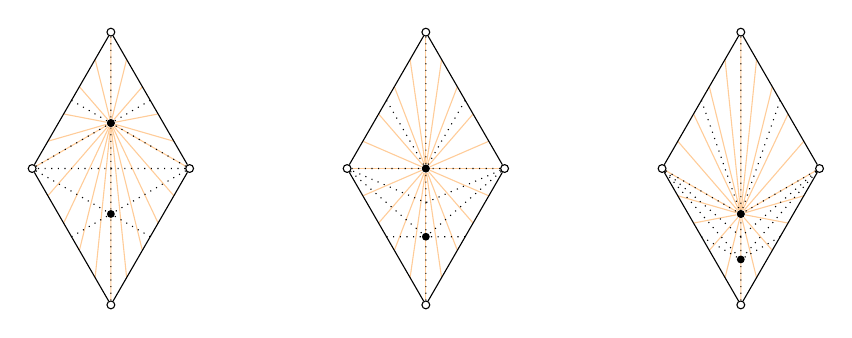
\begin{tikzpicture}[scale=2]
  \pgfmathsetmacro{\y}{sqrt(3)/2}
  \pgfmathsetmacro{\xl}{1/2}

  \def\drawss{
    % Name the vertices of the simplex
    % a
    % / \
    % c - b
    % \ /
    % d
    %
    \node[circle, draw=black, fill=white, inner sep=1pt] (a) at (0,\y) {};
    \node[circle, draw=black, fill=white, inner sep=1pt] (b) at (\xl,0) {};
    \node[circle, draw=black, fill=white, inner sep=1pt] (c) at (-\xl,0) {};
    \node[circle, draw=black, fill=white, inner sep=1pt] (d) at (0,-\y) {};
    \coordinate (mab) at ($.5*(a) + .5*(b)$);
    \coordinate (mac) at ($.5*(a) + .5*(c)$);
    \coordinate (mbd) at ($.5*(d) + .5*(b)$);
    \coordinate (mcd) at ($.5*(d) + .5*(c)$);

    \foreach \rat in {1,2,...,4}{
      \pgfmathsetmacro{\ratfrac}{\rat/5}
      \pgfmathsetmacro{\compratf}{1 - \ratfrac}

      \coordinate (ab\rat) at ($\ratfrac*(a) + \compratf*(b)$);
      \coordinate (ac\rat) at ($\ratfrac*(a) + \compratf*(c)$);
      \coordinate (bd\rat) at ($\ratfrac*(b) + \compratf*(d)$);
      \coordinate (cd\rat) at ($\ratfrac*(c) + \compratf*(d)$);
      \draw[orange!40!white] (ab\rat) -- (dpoint) (ac\rat) --
      (dpoint) (bd\rat) -- (dpoint) (cd\rat) -- (dpoint);
    }

    % Draw the lines from the vertices to the moving point
    \draw[orange!40!white] (a) -- (dpoint) (b) -- (dpoint) (c) -- (dpoint) (d) -- (dpoint);

    \coordinate (baanc) at (0.0, 0.28867513459481287);
    \coordinate (bbanc) at (0.0, -0.8660254037844386);
    \pgfmathsetmacro{\bat}{1}
    \pgfmathsetmacro{\bbt}{0.5}
    \pgfmathsetmacro{\batc}{1-\bat}
    \pgfmathsetmacro{\bbtc}{1-\bbt}


    \node[circle, fill=black, inner sep=1pt] (b1) at ($\bat*(dpoint) + \batc*(baanc)$) {};
    \node[circle, fill=black, inner sep=1pt] (b2) at ($\bbt*(dpoint) + \bbtc*(bbanc)$) {};

    \coordinate (mbc) at ($.5*(b1) + .5*(b2)$);

    \draw[dotted] (a) -- (b1) (b) -- (b1) (c) -- (b1) (mab) -- (b1)
    (mac) -- (b1) (mbc) -- (b1) (b) -- (mbc) -- (c);

    \draw[dotted] (d) -- (b2) (b) -- (b2) (c) -- (b2) (mbd) -- (b2)
    (mcd) -- (b2) (mbc) -- (b2);



    % OK, now to draw the middle line.
    %
    % The middle line gets a special name since we're gonna
    % use the intersections to deform it
    % \path[name path=middle] (b) -- (c);

    % \node[circle, draw=black, fill=white, inner sep=1pt] (bary1) at ($1/3*(a) + 1/3*(b) + 1/3*(c)$) {};

    % First barycenter
    % \def\transpt##1{%

    %   \path[name path=pbd] (bd\rat) -- (sspoint);

    %   \path[name intersections={of=pbd and middle, by=bdi}];

    %   \coordinate (bdidiff) at ($(bdi) - (sspoint)$);

    %   \coordinate (ebdiff) at ($(bd\rat) - (sspoint)$);

    %   \path let \p1 = (bdidiff), \p2 = (ebdiff) in coordinate
    %   (bmid\rat) at ($\x1/\x2*(bd\rat) - \x1/\x2*(dpoint)$);

    %   \coordinate (bmid\rat) at ($(bmid\rat) + (dpoint)$);
    % }


    % Draw boundary of simplex
    \draw (a) -- (b) -- (d) -- (c) -- (a);


  }

  % Start point and endpoint
  % \coordinate (spoint) at (0.2, 0.4);
  % \coordinate (epoint) at (-0.15, -0.3);
  \coordinate (spoint) at (0.0, 0.28867513459481287);
  \coordinate (epoint) at (0.0, -0.28867513459481287);
  % \coordinate (spoint) at (.2, .4);
  % \coordinate (epoint) at (-.15, -.3);
  % \coordinate (spoint) at (v);
  % \coordinate (epoint) at (u);

  \begin{scope}[xshift=-2cm]
    \coordinate (sspoint) at ($(spoint) + (-2.,0.)$);
    \node[circle, fill=black, inner sep=1pt] (dpoint) at ($(sspoint) +
    (0.,0.)$) {};
    \drawss
  \end{scope}

  \begin{scope}[xshift=0cm]
    \coordinate (sspoint) at (spoint);
    \node[circle, fill=black, inner sep=1pt] (dpoint) at
    ($.5*(spoint) + .5*(epoint)$) {};
    \drawss
  \end{scope}

  \begin{scope}[xshift=2cm]
    \coordinate (sspoint) at ($(spoint) + (2.,0.)$);
    \coordinate (epoint) at ($(epoint) + (2., 0)$);
    \node[circle, fill=black, inner sep=1pt] (dpoint) at
    (epoint) {};
    \drawss
  \end{scope}
\end{tikzpicture}
\end{document}
